\documentclass[10pt, a4paper, twocolumn]{article}

% --- PACOTES FUNDAMENTAIS ---
\usepackage[utf8]{inputenc}
\usepackage[T1]{fontenc}
\usepackage[portuguese]{babel}
\usepackage{amsmath, amssymb}
\usepackage{graphicx}
\usepackage{booktabs}
\usepackage[margin=1.5cm, columnsep=0.8cm]{geometry}
\usepackage{hyperref}
\usepackage{caption}
\usepackage{subcaption}
\usepackage{float}
\usepackage[section]{placeins}
\usepackage{microtype}
\setcounter{secnumdepth}{2}

% --- DADOS DO DOCUMENTO ---
\title{\vspace{-1.2cm}\textbf{Análise Estatística Comparativa entre Municípios da PB e do RN: Inferências e Resultados}}
\author{
    Brenno H. A. S. Costa \quad Deivyson H. G. Ribeiro \quad Gustavo H. R. Oliveira \\
    Ítalo O. De Sousa \quad Samuel C. L. Carvalho \\
    \vspace{0.25cm}
    \textit{Universidade Federal da Paraíba (UFPB)} \\
    \textit{Métodos Estatísticos Aplicados às Ciências Tecnológicas}
}
\date{26 de março de 2026}

\begin{document}
\raggedbottom
\maketitle

\begin{abstract}
Este relatório apresenta uma análise comparativa de indicadores socioeconômicos e educacionais em municípios da Paraíba (PB) e do Rio Grande do Norte (RN). Foram utilizadas populações de $N_{PB}=223$ e $N_{RN}=167$ municípios, com amostras aleatórias simples de tamanho $n=30$ por estado. A análise combinou estatísticas descritivas, inspeção gráfica e inferência estatística por testes F e testes t para amostras independentes, ao nível de significância de $\alpha = 0{,}05$. Os resultados indicam ausência de diferença estatisticamente significativa para renda até 1/2 salário mínimo e salário médio formal, mas diferença significativa para o IDEB, favorável à PB no recorte amostral analisado. Em termos substantivos, os achados sugerem similaridade econômica entre as amostras e diferença educacional relevante.
\end{abstract}

\section{Introdução e Metodologia}
\subsection{Dados e amostragem}
A análise de indicadores educacionais e socioeconômicos em nível municipal permite compreender desigualdades regionais e apoiar decisões de políticas públicas. Neste estudo, utilizamos dados do IBGE para PB e RN e adotamos amostragem aleatória simples com reprodutibilidade computacional.

\subsection{Procedimentos inferenciais}
Os procedimentos inferenciais seguiram o conteúdo da disciplina: teste de variâncias (F e, no caso da variável salarial, Levene) e teste t para comparação de médias entre duas amostras independentes. Para cada comparação, também foram reportados intervalos de confiança de 95\%.

\subsection{Fontes de dados e reprodutibilidade}
As bases utilizadas foram extraídas da plataforma IBGE Cidades e Estados. Para atender ao enunciado, os links das amostras selecionadas pelo grupo estão listados abaixo:
\begin{itemize}
    \item Fonte principal (IBGE): \url{https://www.ibge.gov.br/cidades-e-estados.html?view=municipio}
    \item Base PB (planilha): \url{https://docs.google.com/spreadsheets/d/1dbfaJHCybOgAuf_P7Ujg2A0mNr2ZrPImYFe40pVMcD0/edit?gid=0#gid=0}
    \item Base RN (planilha): \url{https://docs.google.com/spreadsheets/d/1pD_gEoSGqGzY_pQOh10qqtEdwjBT8TLFj-rMiI9i-cM/edit?gid=0#gid=0}
    \item Amostra 1 -- PB (n=30): \url{https://docs.google.com/spreadsheets/d/1DqZvB6SAwmrf-EYKcq90RhJL3cMQnZgbkhUaw9i3zws/edit?gid=1430399149#gid=1430399149}
    \item Amostra 2 -- RN (n=30): \url{https://docs.google.com/spreadsheets/d/1FN0oUPgRJUvP-P-CZehLo5ZwqQY48Y_tuhvTvpAc9sM/edit}
    \item Estatísticas descritivas (populações e amostras): \url{https://docs.google.com/spreadsheets/d/1wrH-UWGaOjJV9LqyGwj2e5mrUZGNdGWWSNqd70czbLY/edit?usp=sharing}
\end{itemize}

\section{Estatísticas Descritivas}
\subsection{Explicação}
As medidas de tendência central e dispersão foram calculadas para as variáveis de interesse. A moda foi dispensada devido à natureza contínua das variáveis numéricas.

\subsection{Insights}
Mesmo com médias salariais próximas (PB: 1,8033; RN: 1,8267), os desvios padrão indicam dispersão interna relevante em ambos os estados, consistente com heterogeneidade municipal. Esse padrão reforça que comparações entre estados devem ser acompanhadas por inferência formal, e não apenas por diferenças aparentes de média.

Os valores descritivos de referência estão resumidos na Tabela \ref{tab:descritiva_salario}.

As tabelas completas de estatísticas descritivas (populações e amostras para todas as variáveis) foram disponibilizadas no link de reprodutibilidade apresentado na Subseção 1.3.

% Tabela posicionada ao fim da seção para não interromper a leitura entre 2.1 e 2.2.
\begin{table}[htbp] 
\centering
\caption{Estatísticas descritivas da variável salário médio formal (amostras)}
\label{tab:descritiva_salario}
\begin{tabular}{lcc}
\toprule
\textbf{Métrica} & \textbf{PB} & \textbf{RN} \\
\midrule
Tamanho amostral ($n$) & 30 & 30 \\
Média (SM) & 1,8033 & 1,8267 \\
Desvio padrão & 0,2798 & 0,2586 \\
\bottomrule
\end{tabular}
\end{table}

\FloatBarrier

\section{Análise Gráfica}
\subsection{Explicação}
A variável salário médio mensal foi analisada por histogramas e boxplots (ver Figura \ref{fig:painel_salarios}). Observou-se assimetria positiva em ambas as amostras, com maior heterogeneidade no RN.

\begin{figure}[htbp]
    \centering
    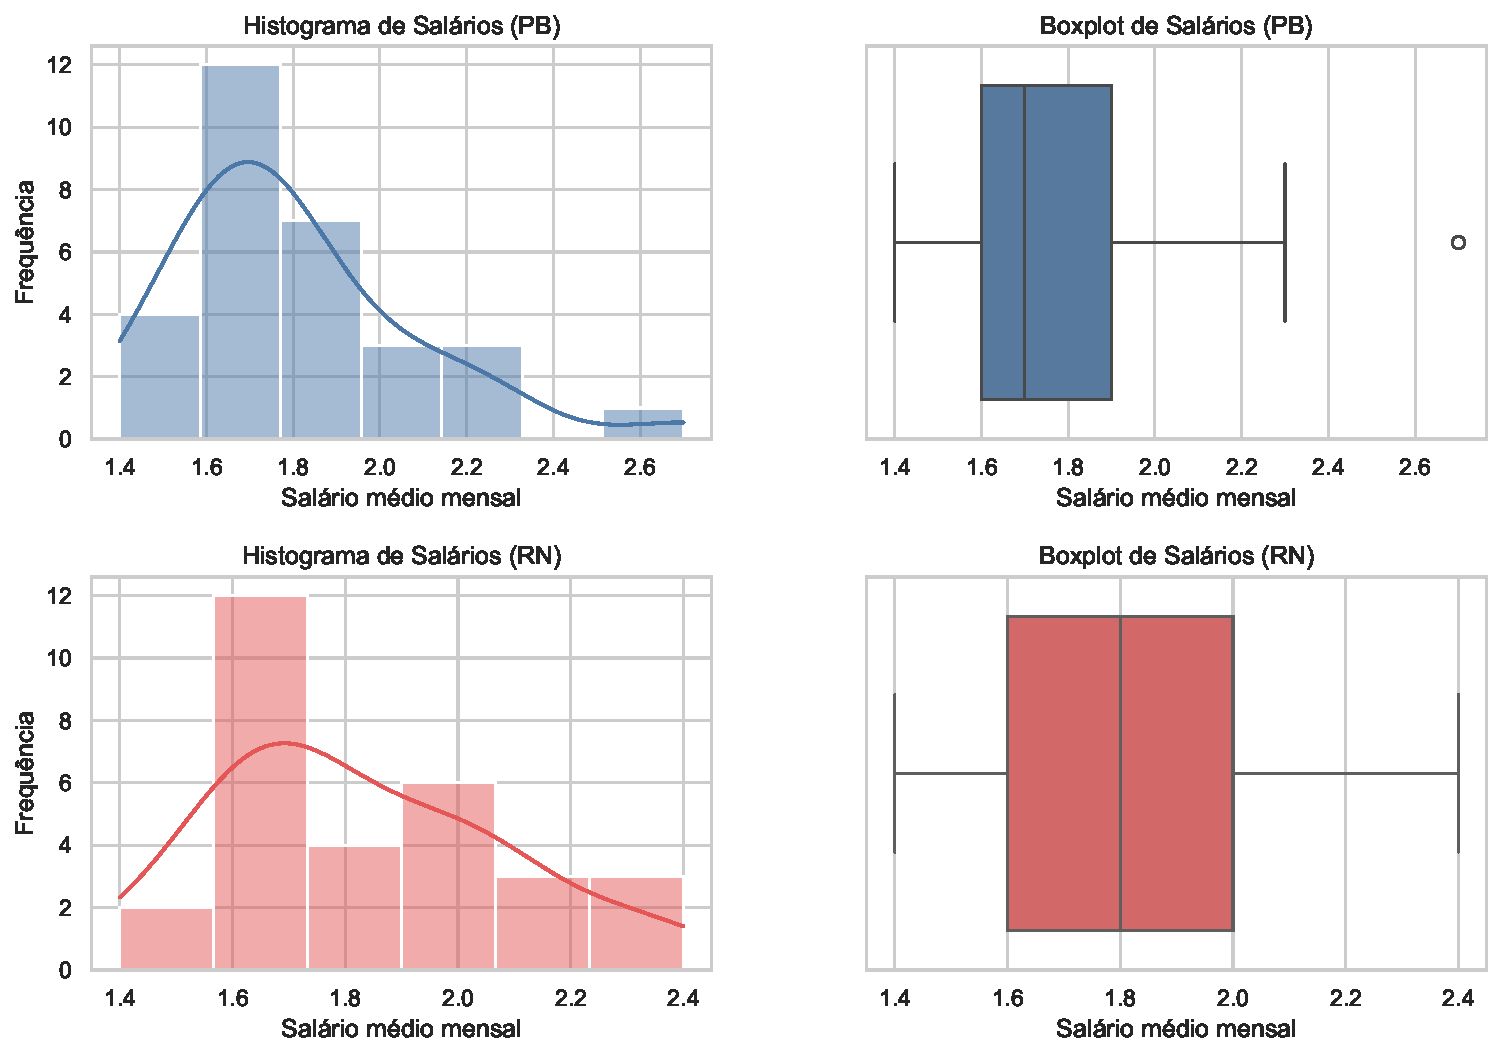
\includegraphics[width=\columnwidth]{figures/painel_salarios.pdf}
    \caption{Distribuição da variável salário médio mensal nas amostras de PB e RN (figura vetorial).}
    \label{fig:painel_salarios}
\end{figure}

\subsection{Insights}
A assimetria à direita indica concentração de municípios em níveis salariais mais baixos e poucos municípios com salários mais altos deslocando a média. Esse comportamento explica por que medianas e quartis são úteis como complemento à média para leitura da distribuição.

\FloatBarrier

\section{Inferência Estatística}
Os resultados completos dos testes de hipóteses estão resumidos na Tabela \ref{tab:inferencia}.

\begin{table}[htbp]
\centering
\caption{Resumo dos resultados inferenciais ($\alpha=0{,}05$)}
\label{tab:inferencia}
\scriptsize
\setlength{\tabcolsep}{2pt}
\begin{tabular}{c p{0.27\columnwidth} c c p{0.23\columnwidth}}
\toprule
\textbf{Ativ.} & \textbf{Variável} & \textbf{Estatística} & \textbf{$p$-valor} & \textbf{Decisão} \\
\midrule
3 & Renda até 1/2 SM (\%) & $t=0,9121$ & 0,3655 & Não rejeita $H_0$ \\
4 & IDEB (anos iniciais) & $t=3,7564$ & 0,0004 & Rejeita $H_0$ \\
5 & Salário médio formal (SM) & $t=-0,3355$ & 0,7385 & Não rejeita $H_0$ \\
\bottomrule
\end{tabular}
\end{table}


\subsection{Proporção municipal de renda até 1/2 salário mínimo}
A diferença média estimada foi de $1{,}0167$ p.p. (PB -- RN), com IC95\% $[-1{,}2147;\ 3{,}2480]$. Como $p=0{,}3655$, não houve evidência estatística de diferença entre os estados ao nível de 5\%.

\textbf{Insight.} Embora a média da PB tenha sido numericamente superior, o intervalo de confiança inclui zero e a evidência amostral não sustenta diferença sistemática entre os estados nesse indicador social.

\subsection{Comparação das médias do IDEB}
A média de IDEB foi maior na PB (5,4138) em comparação ao RN (4,8200). A diferença média foi de $0{,}5938$ ponto, com IC95\% $[0{,}2773;\ 0{,}9103]$. O teste t indicou significância estatística ($p=0{,}0004$).

\textbf{Insight.} Diferentemente dos indicadores econômicos, aqui há evidência robusta de desigualdade entre os estados no recorte amostral. O efeito observado é substantivamente relevante para o contexto educacional municipal.

\subsection{Comparação das médias salariais}
Para salário médio formal, observou-se média de 1,8033 (PB) e 1,8267 (RN). A suposição de variâncias iguais foi sustentada pelo teste de Levene ($p=0{,}8397$), e o teste t apresentou resultado não significativo ($p=0{,}7385$). Em termos inferenciais, os dados não apontam diferença média entre os estados nesse indicador.

\textbf{Insight.} A proximidade das médias e o $p$-valor elevado sustentam a leitura de patamares salariais formais semelhantes entre as amostras de PB e RN.

\FloatBarrier

\section{Discussão Integrada}
\subsection{Síntese dos achados}
Em conjunto, os resultados sugerem um padrão importante: os indicadores de renda e salário formal não diferem estatisticamente entre os estados, enquanto o IDEB apresenta diferença clara em favor da PB. Isso indica que, no recorte analisado, a dimensão educacional não reproduz integralmente o mesmo comportamento da dimensão econômica.

\subsection{Implicações}
Do ponto de vista metodológico, a convergência entre evidências descritivas, gráficas e inferenciais fortalece a consistência dos achados. Em termos aplicados, os resultados apontam maior potencial de ganho analítico em políticas voltadas à educação básica municipal, especialmente na redução de disparidades de desempenho.

\section{Conclusão}
\subsection{Conclusão geral}
Este estudo mostrou convergência entre PB e RN para renda até 1/2 salário mínimo e salário médio formal, mas divergência no IDEB, com evidência de desempenho médio superior da PB no recorte amostral estudado.

\subsection{Limitações e trabalhos futuros}
Como limitações, destacam-se o tamanho amostral, o delineamento transversal e o uso de base secundária com ausências em parte do IDEB. Como trabalhos futuros, recomenda-se ampliar a amostra, incorporar análise temporal e investigar covariáveis associadas ao desempenho educacional municipal (infraestrutura escolar, gasto por aluno, perfil socioeconômico local).

\section{Referências}
\begin{itemize}
    \item IBGE. \textit{Cidades e Estados}. Disponível em: \url{https://www.ibge.gov.br/cidades-e-estados.html?view=municipio}. Acesso em: 22 mar. 2026.
    \item Base de municípios da Paraíba (planilha Google). Disponível em: \url{https://docs.google.com/spreadsheets/d/1dbfaJHCybOgAuf_P7Ujg2A0mNr2ZrPImYFe40pVMcD0/edit?gid=0#gid=0}. Acesso em: 22 mar. 2026.
    \item Base de municípios do Rio Grande do Norte (planilha Google). Disponível em: \url{https://docs.google.com/spreadsheets/d/1pD_gEoSGqGzY_pQOh10qqtEdwjBT8TLFj-rMiI9i-cM/edit?gid=0#gid=0}. Acesso em: 22 mar. 2026.
\end{itemize}

\end{document}